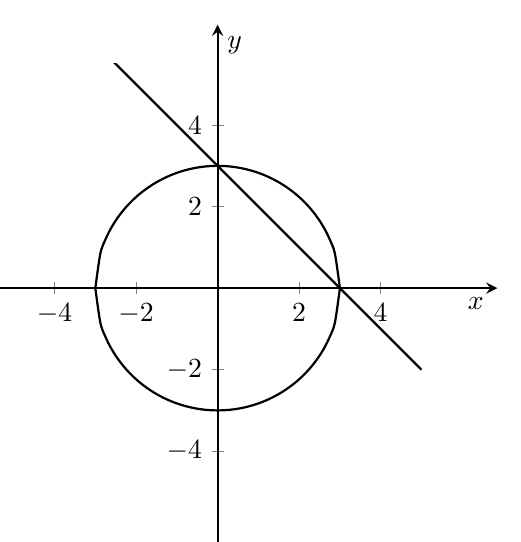
\begin{tikzpicture}
\begin{axis}[ 
xlabel=$x$,
ylabel=$y$,
axis x line=center, xlabel style={anchor=north west},
axis y line=center, ylabel style={anchor=south west},
xmin=-4.5,
xmax=5.9,
ymin=-5.5,
ymax=5.5,
axis line style={thick, shorten > = -0.5cm, shorten < = -0.5cm},
samples=50,
unit vector ratio*=1 1,
]

\addplot [domain=-3:3, thick, black, smooth]{sqrt(9-x^2)};
\addplot [domain=-3:3, thick, black, smooth]{-sqrt(9-x^2)};
\addplot [domain=-5:5, thick, black, smooth,]{3-x};

\end{axis};
\end{tikzpicture}